\clearpage
\section{Methods} \label{sec.methods}
The schema of the proposed method is illustrated in Fig.~\ref{fig.schema}. \smashpp takes as inputs a reference and a target file and produces as output a position file, which is then fed to the \smashpp visualizer to produce an SVG image. This process has eight major stages: (1)~compression of the original target file, based on the model of original reference file, (2)~filtering and segmentation of the compressed file, (3)~reference-free compression of the segmented files, obtained by the previous stage, (4)~compression of the original reference file, based on the model of segmented files obtained by stage~2, (5)~filtering and segmentation of the compressed files, (6)~reference-free compression of the segmented files, that are obtained by the stage~5, (7)~aggregating positions, generated by stages~3 and~6, and (8)~visualizing the positions. The following sections describe the process in detail.

\begin{figure}[!h]
  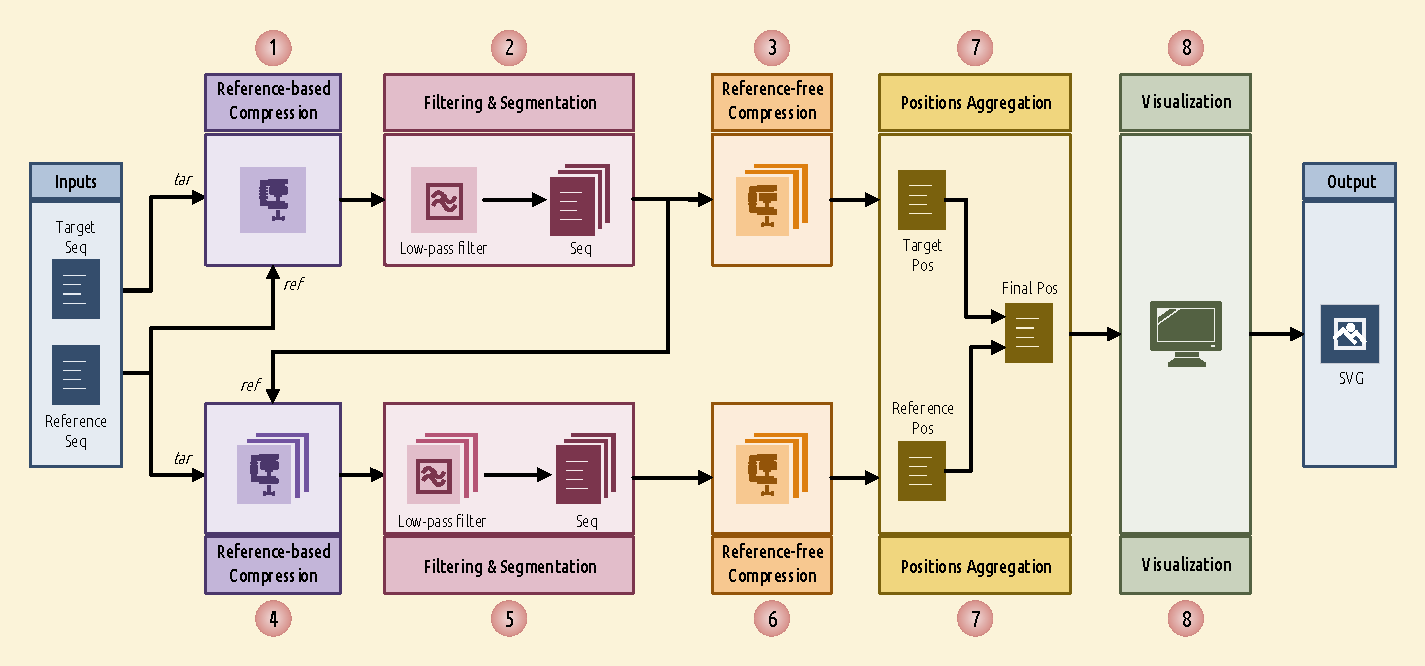
\includegraphics[width=\linewidth]{schema.pdf}
  \caption{The schema of Smash++. The process of finding similar regions in reference and target sequences and also, computing redundancy in each region includes eight stages. Finally, Smash++ outputs a *.pos file that includes the positions of the similar regions, and can be then visualized, resulting in an SVG image.}
  \label{fig.schema}
\end{figure}

\subsection{Data modeling}
\smashpp works on the basis of cooperation between finite-context models (FCMs) and substitutional tolerant Markov models (STMMs). Applying these models on various contexts provides probability and weight values, illustrated in Fig.~\ref{fig.model}a, which are then mixed (by multiplication and addition, shown in Fig.~\ref{fig.model}b) to provide the final probability ($P$) of occurring an input symbol. The following subsections describe FCMs and STMMs in detail.

\begin{figure}[!h]
  \centering
  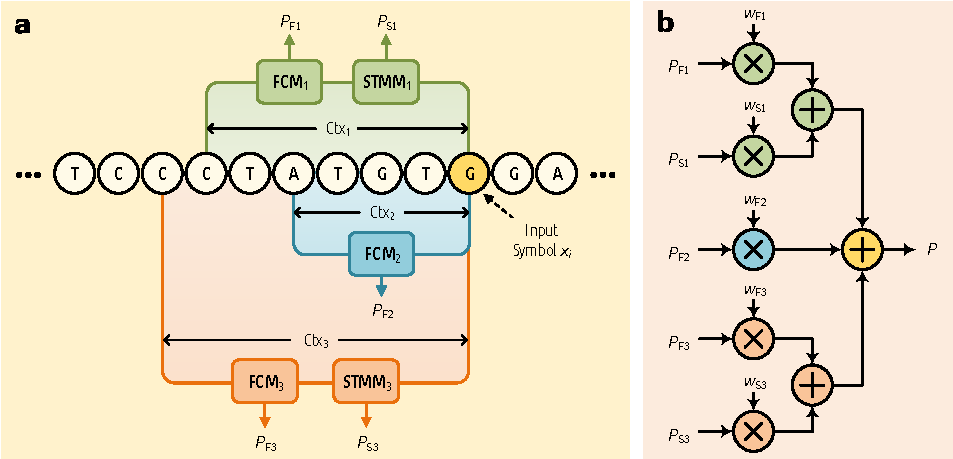
\includegraphics[width=.85\linewidth]{data_model.pdf}
  \caption{Data modelling by Smash++. (a) cooperation between finite-context models (FCMs) and substitutional-tolerant Markov models (STMMs). Note that each STMM needs to be associated with an FCM. (b) probability of an input symbol is estimated by employing the probability and weight values that have been obtained from processing previous symbols.}
  \label{fig.model}
\end{figure}

\subsubsection*{Finite-context model (FCM)}
A finite-context model considers Markov property to estimate the probability of the next symbol in an information source, based on the past $k$ symbols (a context of size $k$)~\cite{sayood2017introduction,hosseini2019ac,pinho2013mfcompress}. Denoting the context as $c_{k,\,i} = s_{i-k} s_{i-k+1}\ldots s_{i-2} s_{i-1}$, the probability of the next symbol $s_i$ in an information source $S$, which is posed at $i$, can be estimated as
\begin{equation} \label{eq.estimate}
  P_m(s_i|c_{k,\,i}) = \frac{N(s_i|c_{k,\,i})+\alpha}{N(c_{k,\,i})+ \alpha|\Theta|},
\end{equation}
in which $m$ stands for model (FCM in this case), $N(s_i|c_{k,\,i})$ shows the number of times that the information source has generated symbol~$s_i$ in the past, $|\Theta|$ denotes size of the alphabet~$\Theta$, $N(c_{k,\,i}) = \sum_{b \in \Theta} N(b|c_{k,\,i})$ represents the total number of events occurred for the context~$c_{k,\,i}$ and $\alpha$ allows to keep a balance between the maximum likelihood estimator and the uniform distribution. Eq.~\ref{eq.estimate} turns to the Laplace estimator, for $\alpha=1$, and also behaves as a maximum likelihood estimator, for large number of events~$i$~\cite{pratas2015alignment}.

\subsubsection*{Substitutional tolerant Markov model (STMM)}
A substitutional tolerant Markov model~\cite{pratas2017substitutional} is a probabilistic-algorithmic model that assumes at each position, the next symbol in the information source is the symbol which has had the highest probability of occurrence in the past. This way, an STMM ignores the real next symbol in the source. Denoting the past $k$ symbols as $c_{k,\,i} = s_{i-k} s_{i-k+1}\ldots s_{i-2} s_{i-1}$, the probability of the next symbol $s_i$, can be estimated as
\begin{equation}
  P_m(s_i|{c'}_{k,\,i}) = \frac{N(s_i|{c'}_{k,\,i})+\alpha}{N({c'}_{k,\,i})+ \alpha|\Theta|},
\end{equation}
where $N$ represents the number of occurrences of symbols, that is saved in memory, and ${c'}_{k,\,i}$ is a copy of the context $c_{k,\,i}$ which is modified as
\begin{equation}
  {c'}_{k,\,i} = \argmax_{\forall b\in \Theta}{P_m(b|{c'}_{k,\,i})}.
\end{equation}

STMMs can be used along with FCMs to modify the behavior of \smashpp in confronting with nucleotide substitutions in genomic sequences. These models have the potential to be disabled, to reduce the number of mathematical calculations and consequently, increase the performance of the proposed method. Such operation is automatically performed using an array of size $k$ (the context size), named history, which preserves the past $k$ hits/misses. Seeing a symbol in the information source, the memory is checked for the symbol with the highest number of occurrences. If they are equal, a hit is saved in the history array; otherwise, a miss is inserted into the array. Before getting to store a hit/miss in the array, it is checked for the number of misses and in the case they are more than a predefined threshold $t$, the STMM will be disabled and also the history array will be reset. This process is performed for each symbol in the sequence.

This example shows the distinction between a finite-context model and a substitutional tolerant Markov model. Assume, the current context at position $i$ is $c_{11,\,i}=\textrm{GGCTAACGTAC}$, and the number of occurrences of symbols saved in memory is $\textrm{A}=10$, $\textrm{C}=12$, $\textrm{G}=13$ and $\textrm{T}=11$. Also, the symbol to appear in the sequence is $\textrm{T}$. An FCM would consider the next context as $c_{11,\,i+1}=\textrm{GCTAACGTACT}$, while an STMM would consider it as ${c'}_{11,\,i+1}=\textrm{GCTAACGTACG}$, since the base $\textrm{G}$ is the most probable symbol, based on the number of occurrences stored in memory.

\subsubsection*{Cooperation of FCMs and STMMs} \label{sec.coop}
When FCMs and STMMs are in cooperation, the probability of the next symbol $s_i$ in an information source $S$, at position $i$, can be estimated as
\begin{equation} \label{eq.coop}
  P(s_i) = \sum_{m\in M_F} P_m(s_i|c_{k,\,i})\;w_{m,\,i} + \sum_{m\in M_S} P_m(s_i|{c'}_{k,\,i})\;{w'}_{m,\,i}, \quad\forall s_i\in S,~1\le i\le |S|,~1\le k\le i-1
\end{equation}
in which $M_F$ and $M_S$ denote sets of FCMs and STMMs, respectively, $P_m(s_i|c_{k,\,i})$ shows the probability of the next symbol estimated by the FCM, $P_m(s_i|{c'}_{k,\,i})$ represents this probability estimated by the STMM, and $w_{m\,i}$ and ${w'}_{m,\,i}$ are weights assigned to each model based on its performance. We have
\begin{align}
  \forall m\in M_F: \quad & w_{m,\,i} \propto (w_{m,\,i-1})^{\gamma_m} P_m(s_i|c_{k+1,\,i-1}),
  \nonumber
  \\[1mm]
  \forall m\in M_S: \quad & {w'}_{m,\,i} \propto ({w'}_{m,\,i-1})^{{\gamma'}_m} P_m(s_i|{c'}_{k+1,\,i-1}),
\end{align}
where $\gamma_m$ and ${\gamma'}_m \in [0,1)$ are forgetting factors predefined for each model. Also,
\begin{equation}
  \sum_{m\in M_F} w_{m,\,i} + \sum_{m\in M_S} {w'}_{m,\,i} = 1.
\end{equation}
By experimenting different forgetting factors for models, we have found that higher factors should be assigned to models that have higher context-order sizes (less complexity) and vice versa. As an example, when the context size $k=6$, $\gamma_m~\mathrm{or}~{\gamma'}_m \simeq 0.9$ and when $k=18$, $\gamma_m~\mathrm{or}~{\gamma'}_m \simeq 0.95$ would be appropriate choices. These values show that forgetting factor and complexity of a model are inversely related.

\subsubsection*{Storing models in memory}
The FCMs and STMMs include, in fact, count values which need to be saved in memory. For this purpose, four different data structures have been employed considering the context-order size $k$, as follows:
\begin{equation*}
  \textrm{data structure} =
  \begin{cases}
    \textrm{table of 64 bit counters},               & 1 \leq k \leq 11 \\
    \textrm{table of 32 bit counters},               & k=12, 13         \\
    \textrm{table of 8 bit approximate counters},    & k=14             \\
    \textrm{Count-Min-Log sketch of 4 bit counters}. & k \ge 15
  \end{cases}
\end{equation*}

\begin{figure}[!h]
  \centering
  \includegraphics[height=.9\textheight]{data_struct.pdf}
  \caption{The data structures used by Smash++ to store the models in memory. (a) table of 64~bit counters that uses up to 128~MB of memory, (b) table of 32~bit counters that consumes at most 960~MB of memory, (c) table of 8~bit approximate counters with memory usage of up to 1~GB and (d) Count-Min-Log sketch of 4~bit counters which consumes up to $\frac{1}{2} w\times d$~B of memory, e.g., if $w=2^{30}$ and $d=4$, it uses 2~GB of memory.}
  \label{fig.struct}
\end{figure}

The table of 64 bit counters, that is shown in Fig.~\ref{fig.struct}a, simply saves number of events for each context. The table of 32 bit counters saves in each position the number of times that the associated context is observed. When a counter reaches to the maximum value $2^{32}-1=4294967295$, all the counts will be renormalized by dividing by two, as shown in Fig.~\ref{fig.struct}b.

The approximate counting is a method that employs probabilistic techniques to count large number of events, while using small amount of memory~\cite{morris1978counting}. Fig.~\ref{alg.approx} shows the algorithm for two major functions associated with this method, \textsc{Update} and \textsc{Query}. In order to update the counter, a pseudo-random number generator (PRNG) is used the number of times of the counter's current value to simulate flipping a coin. If it comes up 0/Heads each time or 1/Tails each time, the counter will be incremented. Fig.~\ref{fig.struct}c shows the difference between arithmetic and approximate counting, and also the values which are actually stored in memory. Note that since an approximate counter represents the actual count by an order of magnitude estimate, one only needs to save the exponent. For example, if the actual count is $8$, we store it in memory as $\log_2 8=3$.
\begin{figure}[h]
  \centering
  \begin{tabular}{|c|}
    \hline
    \begin{minipage}[t]{.5\linewidth}
      \vspace{0pt}
      \begin{algorithmic}[1]
        % \Require table of 8 bit counters
        \Function{\textsc{IncreaseDecision}}{$x$}
        \State \textbf{return} True with probability $\frac{1}{2^x}$, else False
        \EndFunction
        \Statex
        \Function{\textsc{Update}}{$x$}
        \State $c\gets \mathrm{table}[x]$
        \If{$\textsc{IncreaseDecision($c$)}=\mathrm{True}$}
        \State $\mathrm{table}[x]\gets c+1$
        \EndIf
        \EndFunction
        \Statex
        \Function{\textsc{Query}}{$x$}
        \State $c\gets \mathrm{table}[x]$
        \State \textbf{return} $2^c-1$
        \EndFunction
      \end{algorithmic}
      \vspace{2mm}
    \end{minipage}
    \\ \hline
  \end{tabular}
  \caption{Approximate counting update and query.}
  \label{alg.approx}
\end{figure}

The Count-Min-Log Sketch (CMLS) is a probabilistic data structure to save frequency of events in a table by means of a family of independent hash functions~\cite{pitel2015count}. The algorithm for updating and querying the counter is shown in Fig.~\ref{alg.cmls}. In order to update the counter, its current value is hashed with $d$ independent hash functions. Then, a coin is flipped the number of times of the counter's current value, employing a pseudo-random number generator. If it comes up 0/Heads each time or 1/Tails each time, the minimum hashed values (out of $d$ values) will be updated, as shown in Fig.~\ref{fig.struct}d.

The CMLS requires a family of pairwise independent hash functions
$H = \{h: U \to [m]\}$, in which each function $h$ maps some universe $U$ to $m$ bins.
To have this family, we use universal hashing by randomly selecting a hash function from a universal family in which $\forall x,y\in U,~x\neq y:~~P_{h\in H}[h(x)=h(y)]\leq \frac{1}{m}$.
The hash function can be obtained by
\begin{equation}
  h_{a,b}(x)=\left((ax+b)~\bmod p\right)~\bmod m,
\end{equation}
where $p\ge m$ is a prime number and $a$ and $b$ are randomly chosen integers modulo $p$ with $a\neq 0$.

\begin{figure}[h]
  \centering
  \begin{tabular}{|c|}
    \hline
    \begin{minipage}[t]{.55\linewidth}
      \vspace{0pt}
      \begin{algorithmic}[1]
        \Require sketch width $w$, sketch depth $d$, $m$ bins, prime $p\ge m$, randomly chosen integers $a_{1..d}$ and $b_{1..d}$ modulo $p$ with $a\neq 0$
        % independent hash functions $h_{1..d}: U\to \{1..w\}$
        \Statex
        \Function{\textsc{Hash}}{$k, x$} \Comment{Universal hash family}
        \State \textbf{return} $\left((a_k x + b_k)~\bmod p\right)~\bmod m$
        \EndFunction
        \Statex
        \Function{\textsc{MinCount}}{$x$}
        \State $\mathrm{minimum}\gets 15$ \Comment{Biggest 4 bit number}
        \For{$k\gets 1\mathrm{\;to\;}d$}
        \State $h\gets \textsc{Hash}(k, x)$
        \If{$\mathrm{sketch}[k][h] < \mathrm{minimum}$}
        \State $\mathrm{minimum}\gets \mathrm{sketch}[k][h]$
        \EndIf
        \EndFor
        \State \textbf{return} $\mathrm{minimum}$
        \EndFunction
        \Statex
        \Function{\textsc{IncreaseDecision}}{$x$}
        \State \textbf{return} True with probability $\frac{1}{2^x}$, else False
        \EndFunction
        \Statex
        \Function{\textsc{Update}}{$x$}
        \State $c\gets \textsc{MinCount}(x)$
        \If{$\textsc{IncreaseDecision($c$)}=\mathrm{True}$}
        \For{$k\gets 1\mathrm{\;to\;}d$}
        \State $h\gets \textsc{Hash}(k, x)$
        \If{$\mathrm{sketch}[k][h] = c$}
        \State $\mathrm{sketch}[k][h]\gets c+1$
        \EndIf
        \EndFor
        \EndIf
        \EndFunction
        \Statex
        \Function{\textsc{Query}}{$x$}
        \State $c\gets \textsc{MinCount}(x)$
        \State \textbf{return} $2^c-1$
        \EndFunction
      \end{algorithmic}
      \vspace{2mm}
    \end{minipage}
    \\ \hline
  \end{tabular}
  \caption{Count-Min-Log Sketch update and query.}
  \label{alg.cmls}
\end{figure}

\subsection{Finding similar regions}
To find similar regions in reference and target files, a quantity is required for measuring the similarity. We use ``per symbol information content'' for this purpose, which can be calculated as
\begin{equation}
  \label{eq.inf.content}
  I(s_i) = -\log_2 P(s_i)\quad \mathrm{bpb}, \quad\forall s_i\in S,~1\le i\le |S|
\end{equation}
where $P(s_i)$ denotes the probability of the next symbol $s_i$ in the information source $S$, obtained by Equation~\ref{eq.coop}, and also ``bpb'' stands for bit per base.

The information content is the amount of information required to represent a symbol in the target sequence, based on the model of the reference sequence. The less the value of this measure is for two regions, the more amount of information is shared between them, and therefore, the more similar are the two regions. Note that a version of this measure has been introduced in~\cite{pratas2015alignment}, which employs a single FCM to calculate the probabilities. In this paper, however, we exploit a cooperation between multiple FCMs and STMMs for highly accurate calculation of such probabilities.

The procedure of finding similar regions in a reference and a target sequence, illustrated in Fig.~\ref{fig.simil}, is as follows: after creating the model of the reference, the target is compressed based on that model and the information content is calculated for each symbol in the target. Then, the content of the whole target sequence is smoothed by Hann window~\cite{blackman1959particular}, which is a discrete window function given by $w[n]=0.5-0.5\;\cos \left({\frac {2\pi n}{N}}\right)$, where $0\le n\le N$ and length of the window is $N+1$. Next, the smoothed information content is segmented considering a predefined threshold, meaning that the regions with the content greater than the threshold are filtered out. This is carried out for both regular and inverted repeat homologies and at the end, the result would be the regions in the target sequence that are similar to the reference sequence (Fig.~\ref{fig.simil}a). The described phase repeats for all of the target regions found, in the way that after creating the model for each region, the whole reference sequence is compressed to find those regions in the reference that are similar to each of the target regions (Fig.~\ref{fig.simil}b). The final result would have the form of Fig.~\ref{fig.simil}c.

\begin{figure}[!h]
  \centering
  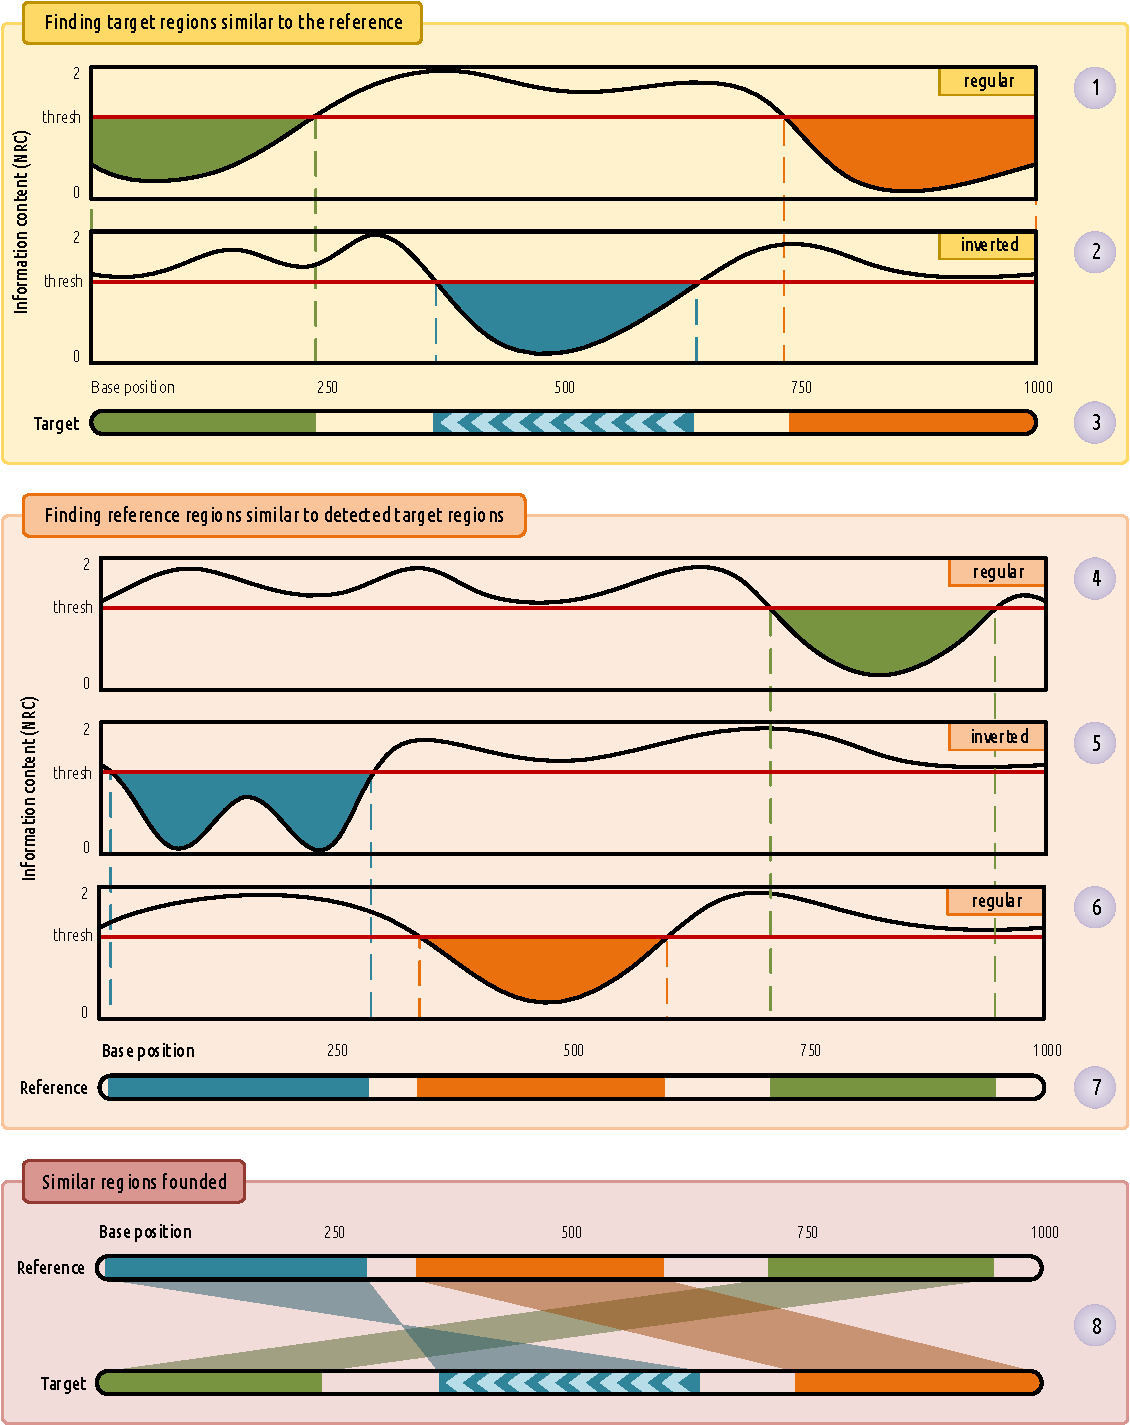
\includegraphics[width=.95\linewidth]{simil.pdf}
  \caption{Finding similar regions in reference and target sequences. Smash++ finds, first, the regions in the target that are similar to the reference, and then, finds the regions in the reference that are similar to the detected target regions. This procedure is performance for both regular and inverted homologies.}
  \label{fig.simil}
\end{figure}

\subsection{Computing complexities}
After finding the similar regions in reference and target sequences, we evaluate redundancy in each region, knowing that it is inversely related to Kolmogorov complexity, i.e., the more complex a sequence is, the less redundant it will be~\cite{hosseini2018cryfa}. The Kolmogorov complexity, $K$, of a binary string $s$, of finite length, is the length of the smallest binary program $p$ that computes $s$ in a universal Turing machine and halts. In other words, $K(s)=|p|$ is the minimum number of bits required to computationally retrieve the string $s$~\cite{turing1936on,li2009an}.

The Kolmogorov complexity is not computable, hence, an alternative is required to compute it approximately. It has been shown in the literature that a compression algorithm can be employed for this purpose~\cite{zenil2015two,antao2018kolmogorov,faloutsos2007on}. In this paper, we employ a reference-free compressor to approximate the complexity and consequently, the redundancy of the found similar regions in the reference and the target sequences. This compressor works based on cooperation of FCMs and STMMs, which is described in detail in Section~\ref{sec.coop}. Note that the difference between reference-based and reference-free version of such compressor is that in the former mode, a model is first created for the reference sequence and then, the target sequence is compressed based on that model, while in the latter mode, the model is progressively created at the time of compressing the target sequence.